\documentclass{article}
\usepackage[utf8]{inputenc}
\usepackage[francais]{babel}
\usepackage{array}
\usepackage{graphicx}
\usepackage{fullpage}
\usepackage[svgnames]{xcolor}
\usepackage{color}
\usepackage{fourier}
\usepackage{pifont}

\newcommand*{\rotrt}[1]{\rotatebox{90}{#1}} % Command to rotate right 90 degrees
\newcommand*{\rotlft}[1]{\rotatebox{-90}{#1}} % Command to rotate left 90 degrees

\newcommand*{\titleBC}{\begingroup % Create the command for including the title page in the document
\centering % Center all text

\def\CP{\textit{\Huge Rapport Projet Ontologies et Web sémantique}} % Title

\settowidth{\unitlength}{\CP} % Set the width of the curly brackets to the width of the title
\textcolor{FireBrick}{\CP} \\[\baselineskip] % Print title
{\color{Grey}\Large "Ontologie des musées et application TrouverUnMusée.fr"} \\
% Tagline or further description
\endgroup}

\definecolor{lg}{rgb}{0.9,0.9,0.9}

\let\oldv\verbatim
\let\oldendv\endverbatim

\def\verbatim{\setbox0\vbox\bgroup\oldv}
\def\endverbatim{\oldendv\egroup\fboxsep0pt \colorbox[gray]{0.9}{\usebox0}\par}

\setlength\parindent{0cm}

%%%% Le Document %%%%

\begin{document}

\begin{table}[h]
    \begin{center}
    \begin{tabular}{ >{\centering\arraybackslash}m{1.5in} >{\arraybackslash}m{4in} }

    \vspace{5mm} \includegraphics[width=2cm]{logo.png} & \vspace{9mm} Ce projet
    a été réalisé dans le cadre du cours de d'Ontologies et Web
    sémantique du Master 2 Pro. GI. par \textbf{Johan GIRARD}, \textbf{Pierre
    ODIN} et \textbf{Abdourahamane TOURÉ}.

  \end{tabular}

  \label{tabular:UKJPNdata}
  \end{center}
\end{table}

\hrule\hrule

\vspace{1.5cm}

\titleBC

\vspace{1cm}

\section{Partie 1 : L’ontologie et les données}

\subsection{Jeu de données}

Le fichier de données sur lequel nous nous sommes basé pour créer notre
ontologie et notre application contient la \textbf{liste des Musées de France
en 2012}. Ces données sont disponibles sur le site \texttt{data.gouv.fr}
(à l'adresse suivante :
\textit{https://www.data.gouv.fr/fr/datasets/liste-et-localisation-des-musees-de-france/}).
Ce fichier contient une liste d'environ 1200 musées en indiquant pour chacun
d'entre eux différentes informations comme son  nom, sa localisation, ses
horaires d'ouverture, etc\ldots

\subsection{L'ontologie (protege)}

L'entité principale de notre ontologie est un \texttt{Musée}. Elle est
équivalente à l'entité \texttt{Museum} de l'ontologie \texttt{schema}
(\texttt{http://schema.org/}). Les entités suivantes permettent de caractériser
un \texttt{Musée} : 
\begin{itemize}
  \item \texttt{Adresse} qui est liée aux entités \texttt{Ville},
\texttt{Département} et \texttt{Région}. Ces entités sont
équivalentes a des entités de l'ontologie \texttt{igeo}
(\texttt{http://rdf.insee.fr/def/geo\#}) et sont des sous-classe de l'entité
\texttt{Localisation}.
  \item \texttt{Thème}
  \item \texttt{SiteWeb} (équivalente à
l'entité \texttt{WebSite} de l'ontologie \texttt{schema})
\item \texttt{HoraireOuverture} , \texttt{OuvertureNocture}
, \texttt{FermetureAnnuelle} , \texttt{DateRéouverture} (un musée ayant une date
de ré-ouverture est un musée actuellement en fermeture prolongée). Ces entités
sont des sous-classe de l'entité \texttt{Période}.
\end{itemize}

\vspace{0.3cm}

L'entité \texttt{MuséeAvecThème} est une sous-classe de \texttt{Musée} qui
regroupe les musées ayant un thème défini. L'entité \texttt{MuséeDisponible} est
une autre sous-classe de \texttt{Musée} qui regroupe les musées qui ne sont
pas actuellement en fermeture prolongée.

\vspace{0.3cm}

Toutes les propriétés sont \texttt{Asymmetric} et \texttt{Irreflexive}.
Certaines propriétés sont \texttt{Fonctional} et d'autres sont
\texttt{Inverse Fonctional} (respectivement notées \texttt{(F)} et \texttt{(IF)}
dans le schéma de l'ontologie ci-après).

\paragraph{\starredbullet} Nous avions également complété l'ontologie avec une
propriété nommée \texttt{estVilleDeLaRégion} qui utilisait l'option
\texttt{SubPropertyOf (Chain)} mais nous avons dû la supprimer car elle
bloquait l'utilisation du raisonneur.

\newpage

Le schéma en trois parties de l'ontologie des musées réalisée est le suivant :

\begin{center}
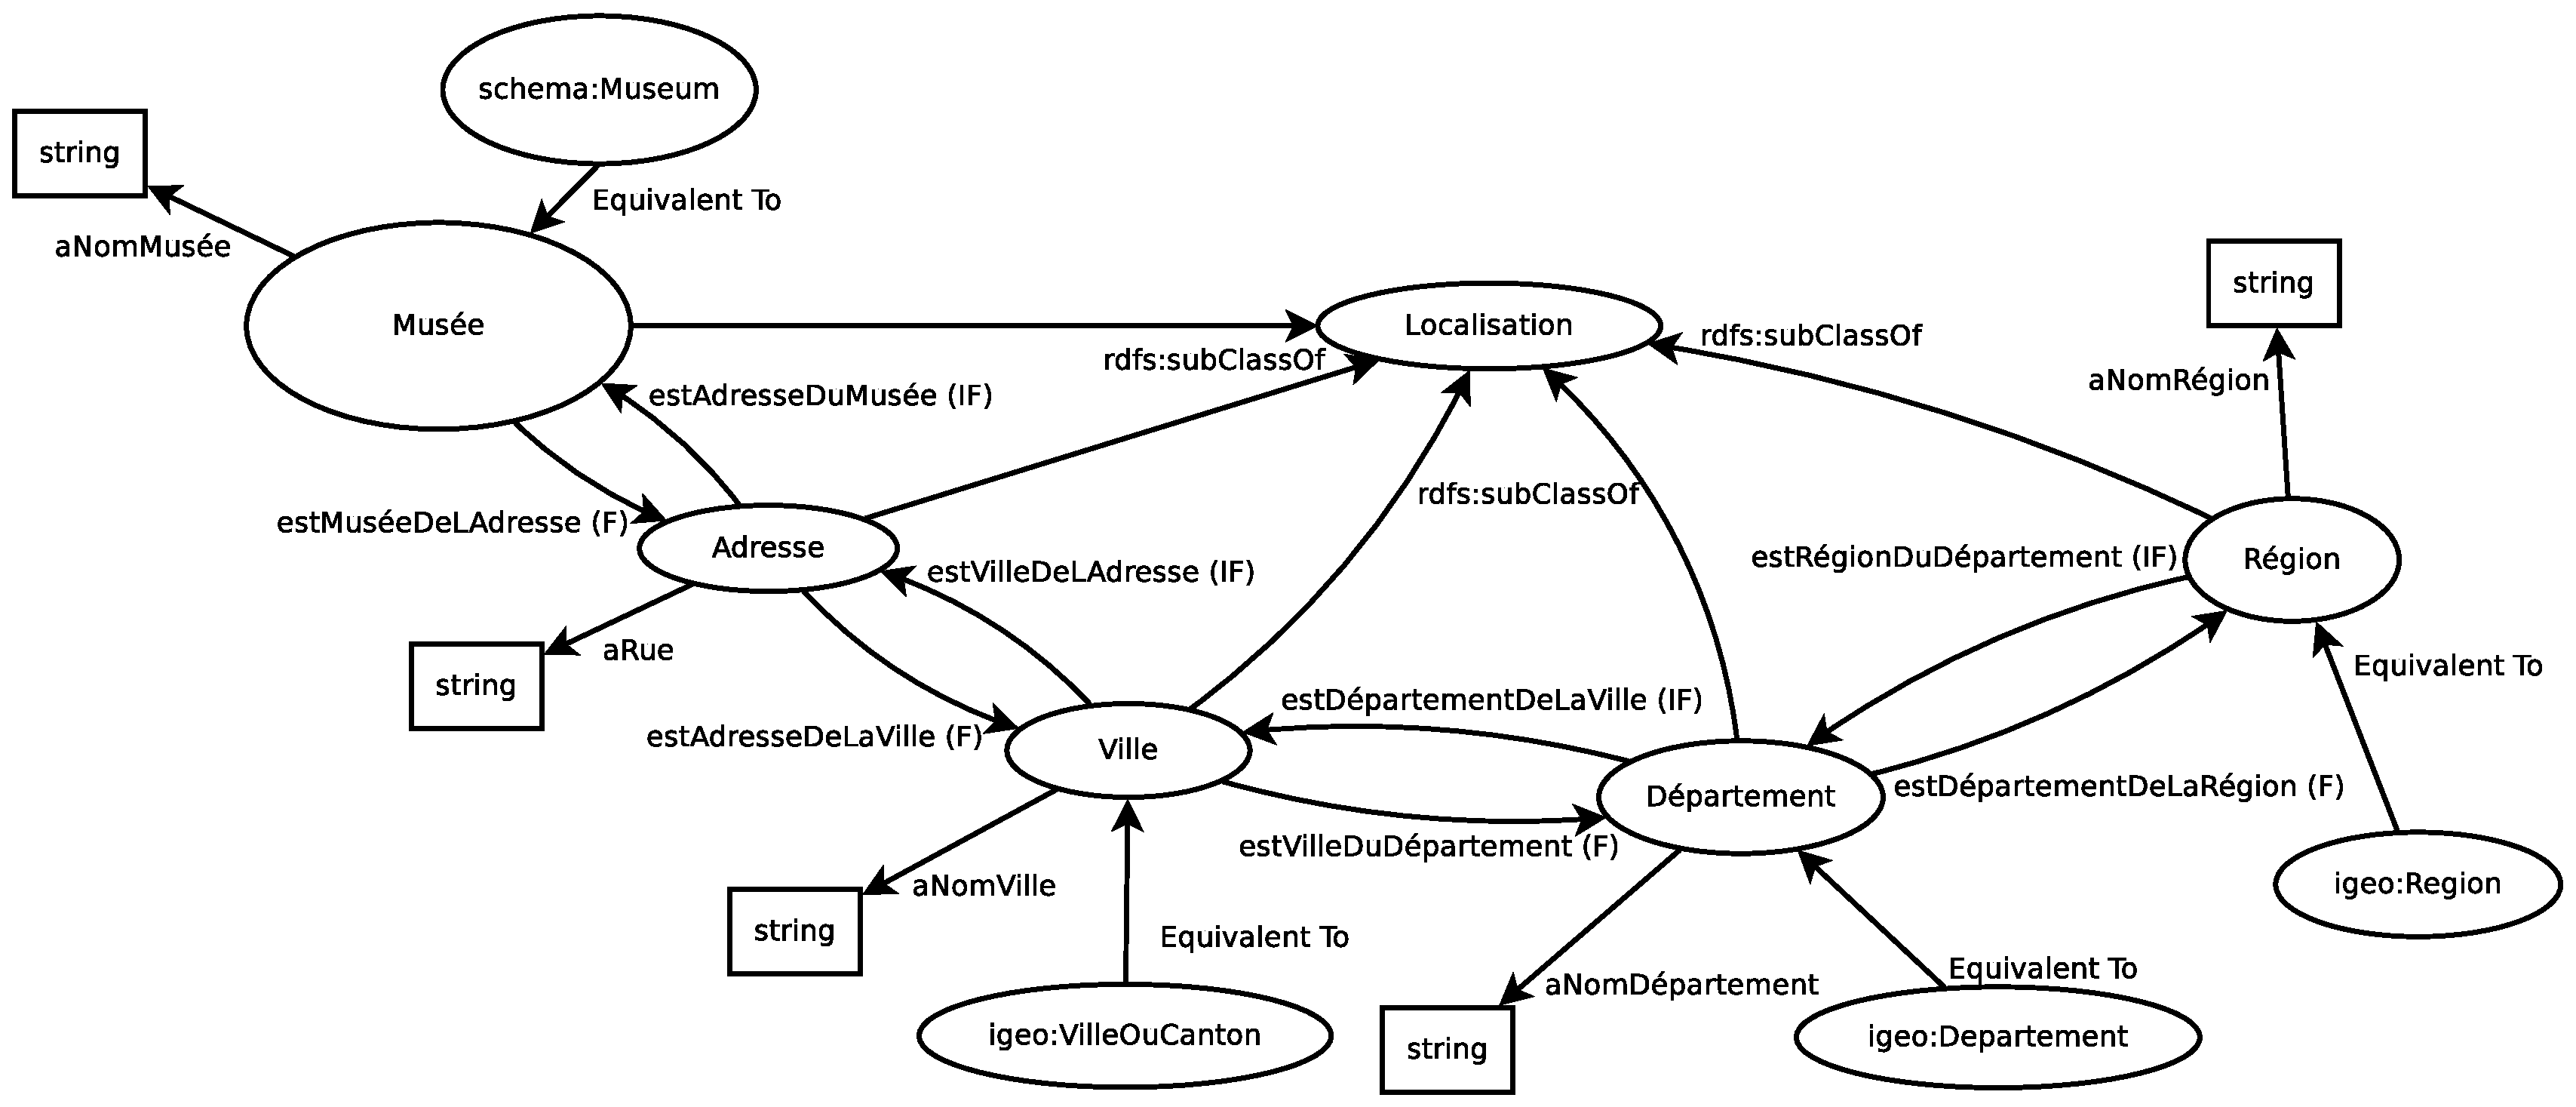
\includegraphics[width=16cm]{Diagramme1.eps}
\end{center}
\vspace{0.3cm}
\begin{center}
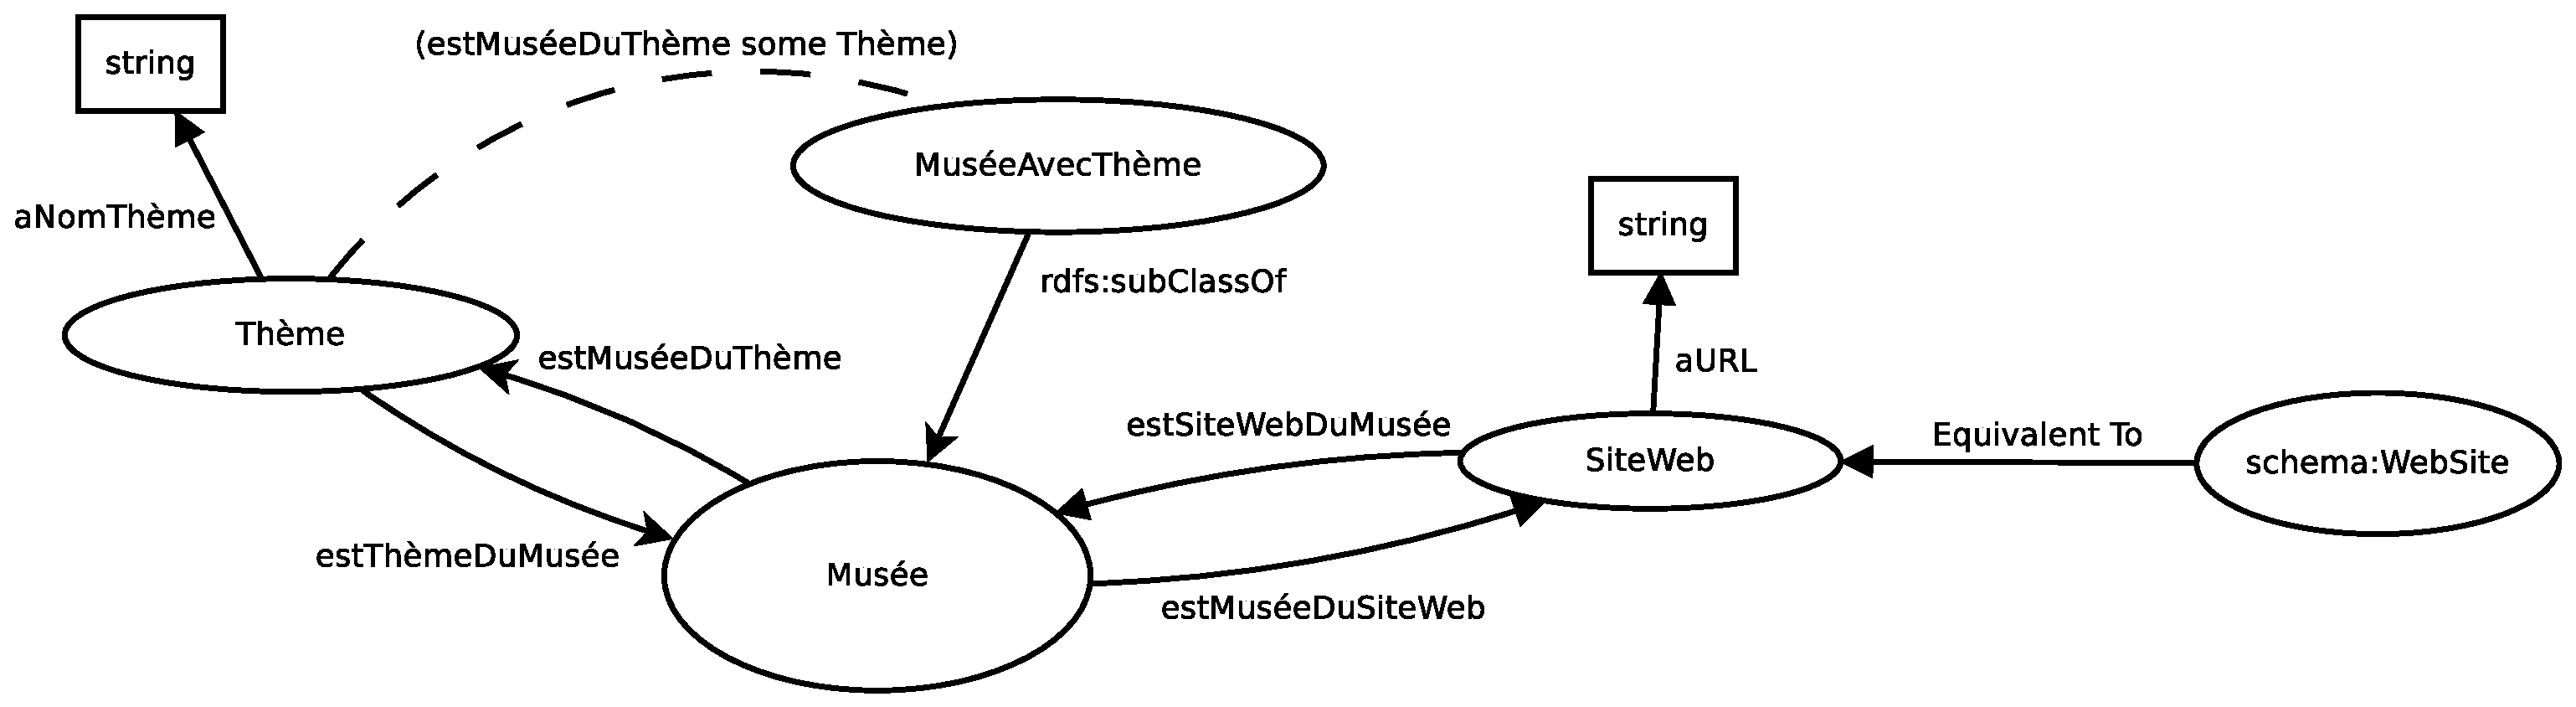
\includegraphics[width=16cm]{Diagramme2.eps}
\end{center}
\vspace{0.3cm}
\begin{center}
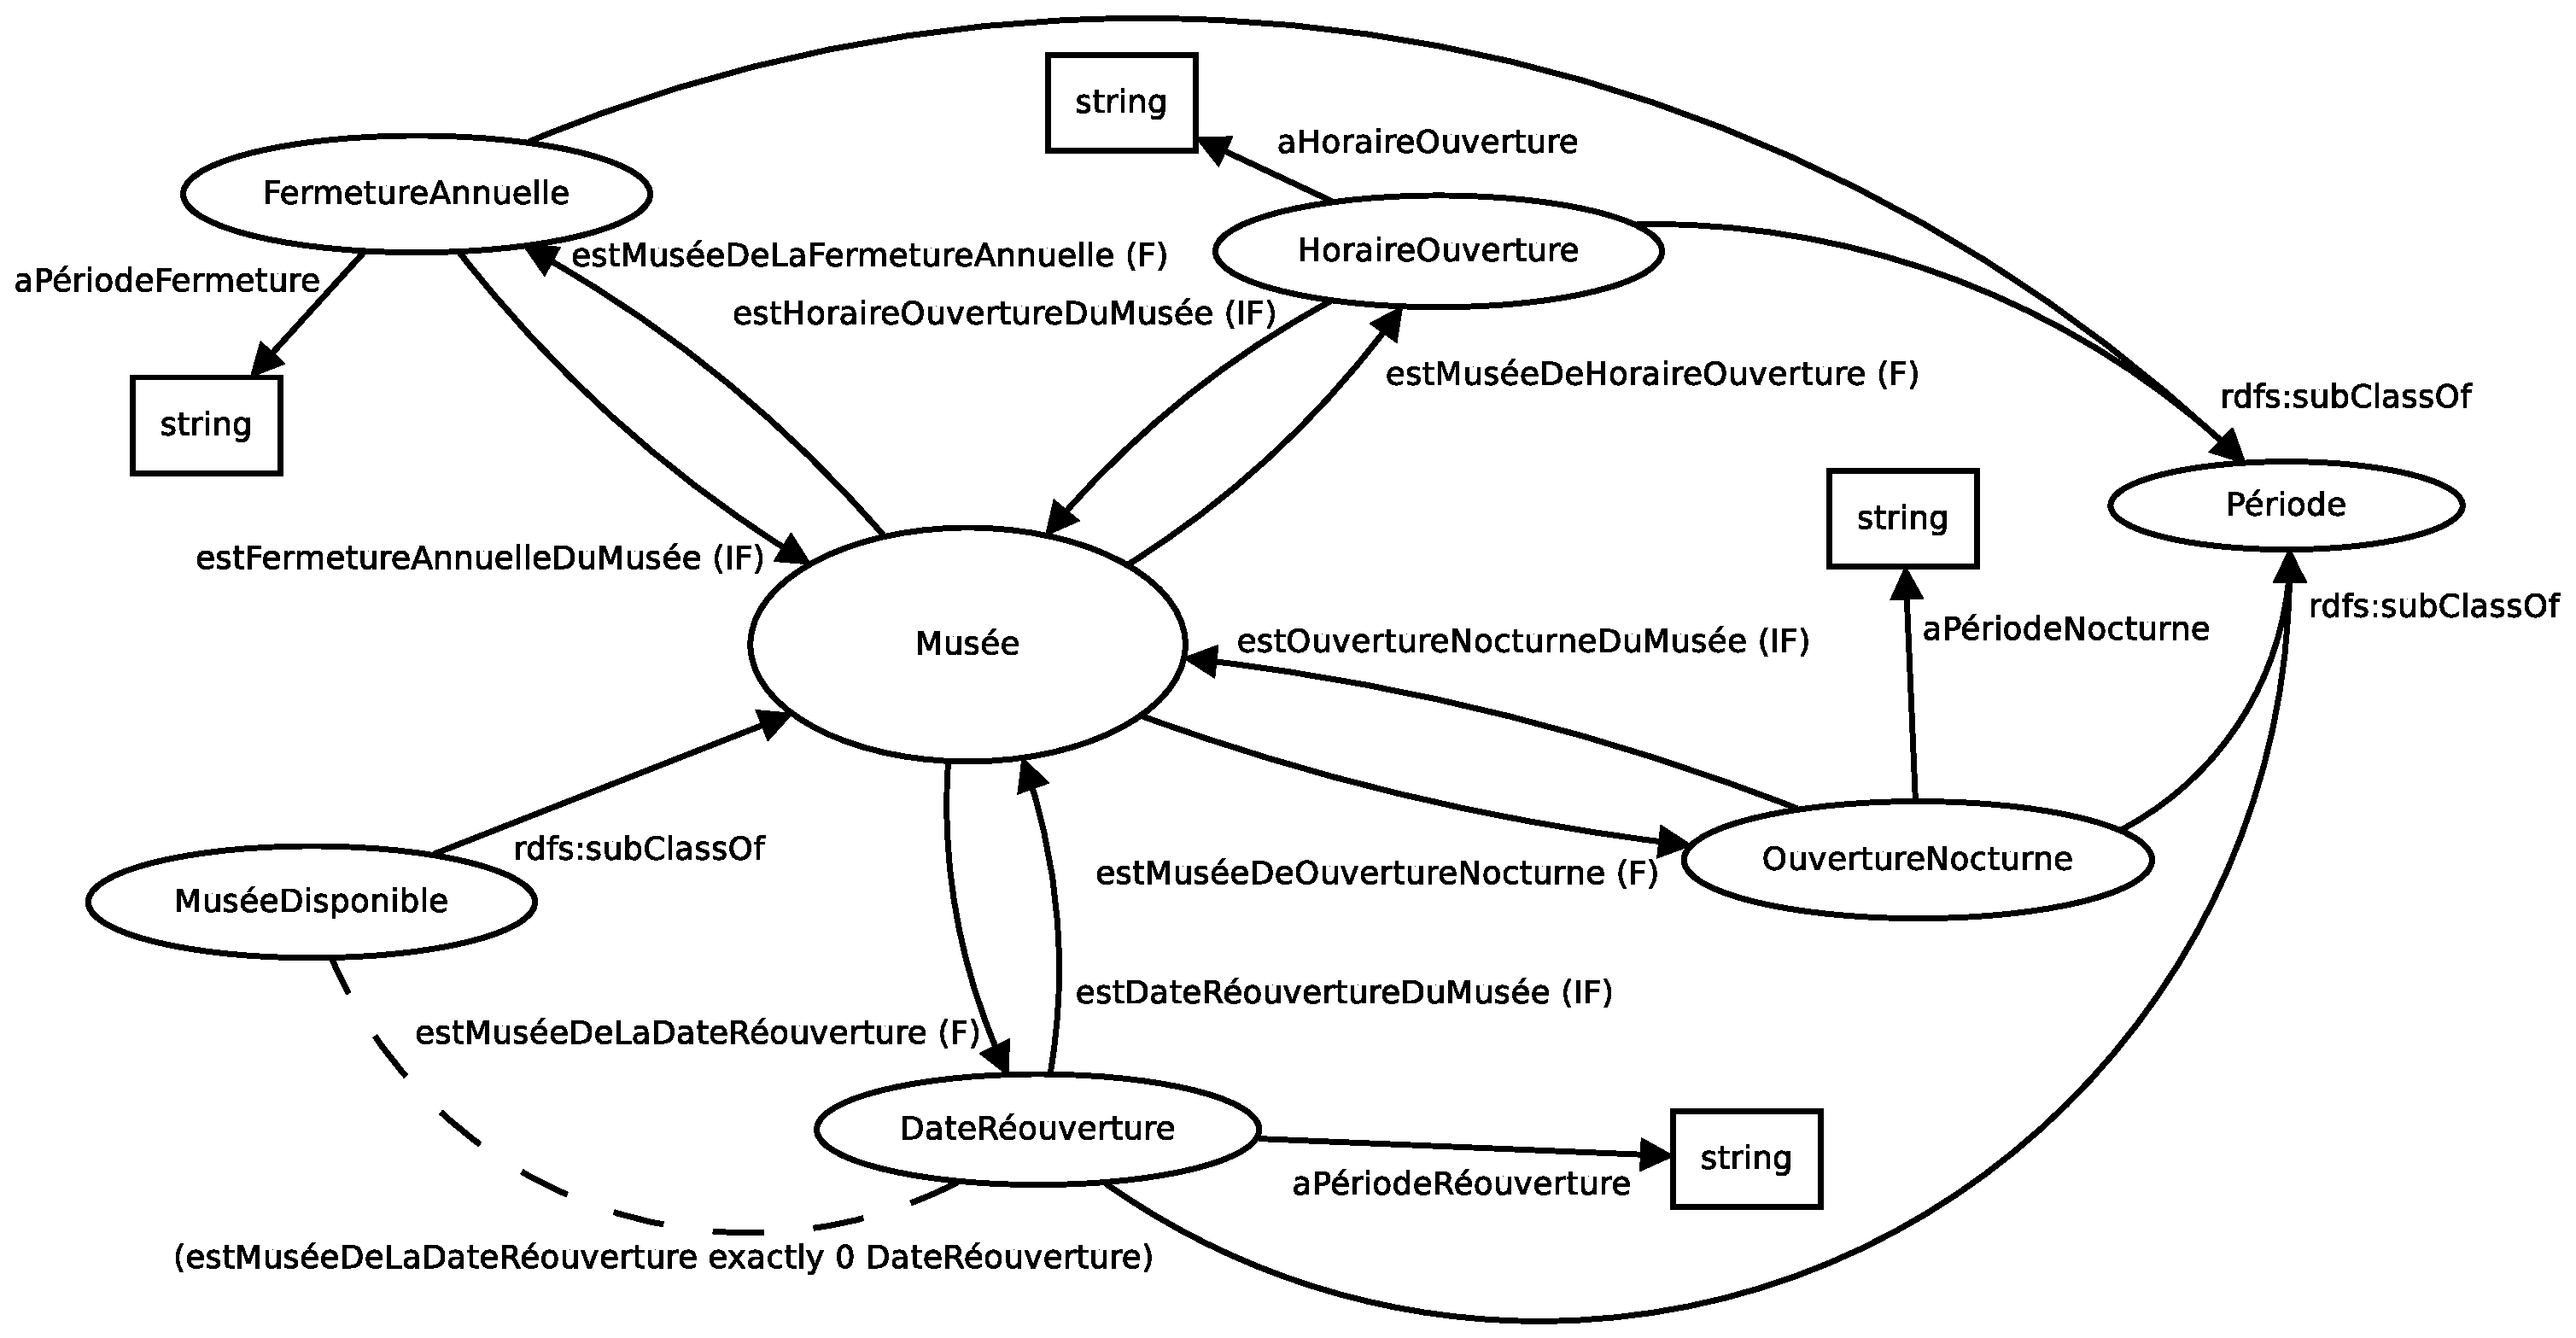
\includegraphics[width=16cm]{Diagramme3.eps}
\end{center}

\subsection{Importation des données}

Nous avons utilisé notre propre programme \texttt{Java} pour peupler
l'ontologie. La première étape a consisté à ajouter des individus avec un
minimum de propriétés à l'ontologie. La seconde étape a consisté à
utiliser le raisonneur de \texttt{protege} pour compléter les propriétés des
individus et généré un fichier \texttt{musee.owl} contenant l'ontologie peuplée
au format \texttt{Turtle}.

\vspace{0.3cm}

L'ensemble des classes \texttt{Java} utilisées sont fournies à titre indicatif.
Elle se trouvent dans le package \texttt{genowl}. De plus, le fichier de données
utilisé n'étant pas uniforme, nous avons dû effecter des modifications ``à la
main" sur ce fichier. Enfin, des modifications ont également été éffectuées sur
le fichier \texttt{musee.owl} à la fin du processus.

\subsubsection{Génération via un programme Java}

Nous avons commencé par générer des identifiants pour les valeurs des
attributs. Par exemple, pour l'attribut \textit{Département}, le BAS-RHIN
correspond à \texttt{D\_32}. Nous avons ensuite associé chaque musée à un
identifiant en rajoutant par exemple une colonne \texttt{ID\_DEP} dans le
fichier de données.
Cette étape a été répété pour plusieurs attributs (région, ville, horaire d'ouverture, etc\ldots).
L'étape suivante à consisté à générer le code \texttt{Turtle} des individus en
indiquant les propriétés nécéssaires (par exemple : individu \texttt{D\_32} de
type \texttt{Département} avec la propriété \texttt{estDépartementDeRégion
R\_10} et \texttt{aNomDépartement "BAS-RHIN"}). Enfin, nous avons généré les
individus de la classe \texttt{Musée} en ajoutant les propriétés faisants le
lien avec les individus précédemments créés.

\vspace{0.3cm}

Un traitement particulier a été fait pour l'entité \texttt{Thème} puisque le
thème de chaque musée est extrait, dans la mesure du possible, du nom du musée.

\subsubsection{Inférences dans protege}

Les différents parties de code \texttt{Turtle} générées avec notre programme
\texttt{Java} ont ensuite été regroupées dans le fichier \texttt{musee.owl}
contenant la structure de l'ontologie (définition des classes et des propriétés). Nous avons alors
utilisé le raisonneur \texttt{HermiT} pour inférer les propriétés manquantes
: \texttt{domain}, \texttt{range}, les propriétés inverses (\texttt{inverseOf}),
etc\ldots

\vspace{0.3cm}

Nous avons corrigé les caractéristiques des propriétés générées par
le raisonneur. En effet, le raisonneur avait ajouté pour une raison inconnue la
caractéristique \texttt{Transitive} à certaines propriétés alors qu'aucune des
propriétés de l'ontologie n'est transitive.

\vspace{0.3cm}

Pour finir, nous avons ajouté au fichier \texttt{musee.owl} des correspondances
entre nos entités et du vocabulaire existant (trouvé sur
\texttt{http://lov.okfn.org/dataset/lov/}).


\section{Partie 2 : Intégration de l'ontologie dans une application Java}

\subsection{Type de l'application}

Nous avons développé une application de type \texttt{web-app}. Pour ceci, nous
nous sommes reposés sur une architecture MVC et l'utilisation de Tomcat. De plus,
afin d'effectuer nos requêtes SPARQL nous utilisons le framwork Apache Jena.
Pour simplifier le développement, nous avons travaillé sur un projet Eclipse,
aussi si vous souhaitez exécuter l'application la démarche à suivre est la
suivante :
\begin{itemize}
  \item Importer le projet dans votre Eclipse.
  \item Ajouter un serveur d'exécution Tomcat à votre projet (Tomcat 8).
  \item Exécuter le projet, le serveur se lance et vous aurez alors accès au
  projet à la page \texttt{localhost:8080/WebOWL/}.
\end{itemize}
Si vous exécutez le projet sur une machine connectée au réseau de l'UFR ou
utilisant un proxy, il est possible que les requêtes SPARQL vers DBPedia ne
fonctionnent pas. Pour pallier à ce problème, une solution possible est de
paramétrer la variable \texttt{proxy\_on} de la classe
\texttt{jena.RequêteDBpedia}.

\subsection{Fonctionnalités}

\subsubsection{Recherche}

Notre application est un moteur de recherche de musées. Elle permet de
rechercher des musées suivants différents critères. Les critères de recherches
sont utilisables en concurence (union des résultats filtrés) et sont les
suivants :
\begin{itemize}
  \item recherche par \textbf{Nom} : vous pouvez rechercher les musées dont le
  nom contient le mot spécifié. La requête SPARQL traitant cette
  recherche utilise un \texttt{FILTER} sur les résultats.
  \item recherche par \textbf{Régions} et/ou par \textbf{Départements} et/ou par
  \textbf{Villes} :
  vous pouvez rechercher des musées suivant plusieurs localisations (plusieurs
  régions, départements ou villes). La requête SPARQL traitant cette recherche
  utilise des \texttt{UNION}. De plus, un système d'auto-complétion a été mis 
  en place pour améliorer l'expérience utilisateur.
  \item recherche par \textbf{Thème} : vous pouvez rechercher les musées dont le
  thème contient le mot spécifié. La requête SPARQL traitant cette
  recherche utilise un \texttt{FILTER} sur les résultats.
\end{itemize}
A titre d'information, la création de ces requêtes SPARQL se trouve dans la
classe \texttt{jena.RequêteMusée}. Enfin, la capture d'image suivante détaille
la fonctionnalité de recherche de notre outil.
\begin{center}
\includegraphics[width=8cm]{trouveMuseeRecherche.png}
\end{center}

\subsubsection{Résultats de recherche}

Une fois la recherche demandée, une ou plusieurs requêtes SPARQL sont générées
et exécutées. Un traitement d'union (en Java) est ensuite mis en place pour
fournir un résultat cohérent. En outre, les résultats de la recherche sont
formulés sous forme d'un tableau contenant le nom du musée, sa région 
(lien vers fiche Région DBPedia), son département et sa ville. De plus, chacune des colonnes est
ordonnable par valeur ascendante ou descendante. Pour réaliser ce tri, nous
rajoutons suivant la demande des \texttt{ORDER BY} sur les requêtes SPARQL.

A titre d'information, la création de ces requêtes SPARQL se trouve dans la
classe \texttt{jena.RequêteMusée}. Enfin, la capture d'image suivante détaille
la fonctionnalité d'affichage d'une recherche de notre outil.
\begin{center}
\includegraphics[width=14cm]{trouveMuseeResultat.png}
\end{center}


\subsubsection{Fiche Région (DBpedia)}

Nous avons mis en place un lien entre notre ontologie et les données de DBpedia
en proposant une Fiche Région. Cette fiche propose plusieurs informations sur la
région : un résumé, la préfecture, la superficie, la population et le site web
de la région. Chacune de ces informations sont extraites de BDpedia.

\vspace{0.3cm}

Pour faire le lien entre notre ontologie et DBpedia, nous utilisons le nom de la
région de notre ontologie (\texttt{aNomRégion}) qui correspond à un
\texttt{rdfs:label} de la région correspondante dans DBpedia (qui appartient à
la classe \texttt{AdministrativeRegion}).
Cette façon de faire le lien nous a obligé à faire une première requête SPARQL
qui récupère le nom et une seconde qui intérroge DBpedia car nous avions un
problème de type de string (\texttt{@fr} est différent de \texttt{xds:string}).
Il aurait été plus judicieux de faire le lien directement entre les individus dans notre ontologie.

\vspace{0.3cm}

La classe \texttt{requêteDBpedia.java} du package \texttt{jena} est utilisé pour
cette fonctionnalité. On peut également noter que la requête interrogeant
DBpedia utilise un filtre pour récuperer un résumé en français (\texttt{FILTER(
lang(?res) = "fr" )}).

\begin{center}
\includegraphics[width=14cm]{trouveMuseeRegion.png}
\end{center}

\subsubsection{Fiche Musée}

TODO

\section{Répartition du travail}

Nous avons travaillé tous ensemble sur le projet sans faire une répartition
stricte des différentes parties. Cependant, le travail de Johan GIRARD s'est un
peu plus porté sur la partie requêtes SPARQL et aux traitements
des résultats, celui de Pierre ODIN sur la création de l'ontologie dans protege et la génération d'individus et
enfin, Abdourahamane TOURÉ s'est plus intéressé à la mise en place de
l'application et aux fonctionnalités DBpedia et Google Map.


\end{document}